\documentclass{beamer}
\usepackage{alltt} 
\usetheme{Warsaw}
\usepackage{xfrac}
\usepackage{blkarray}
% HERE ARE SOME USEFUL PACKAGES. IF YOU DON'T WANT TO USE THEM COMMENT THEM OUT
\usepackage{graphicx}
\usepackage{amsmath}
\usepackage{hyperref}
\usepackage{amssymb}
\usepackage{psfrag}
\usepackage{color,xcolor}
\usepackage{bm}
\usepackage{geometry}
\usepackage{algorithm2e}
\definecolor{light-gray}{gray}{0.8}

\setbeamertemplate{navigation symbols}{}%remove navigation symbols
\title{Body Sensor Networks}
\author{Chris Mower, Kuo Wong}
\date{}
\titlegraphic{
\includegraphics[width=\textwidth,height=.5\textheight]{uMusev4}}

\definecolor{myred}{rgb}{.6667,.1176,.1373}

\setbeamercolor{frametitle}{fg=white}


\setbeamercolor{alerted text}{fg=orange}
\setbeamercolor{background canvas}{bg=myred}
\setbeamercolor{block body alerted}{bg=black text.bg!90!black}
\setbeamercolor{block body}{bg=normal text.bg!90!black}
\setbeamercolor{block body example}{bg=normal text.bg!90!black}
\setbeamercolor{block title alerted}{use={normal text,alerted text},fg=alerted text.fg!75!normal text.fg,bg=normal text.bg!75!black}
\setbeamercolor{block title}{bg=blue}
\setbeamercolor{block title example}{use={normal text,example text},fg=example text.fg!75!normal text.fg,bg=normal text.bg!75!black}
\setbeamercolor{fine separation line}{}
\setbeamercolor{frametitle}{fg=white}
\setbeamercolor{item projected}{fg=black}
\setbeamercolor{normal text}{bg=black,fg=white}
\setbeamercolor{palette sidebar primary}{use=normal text,fg=normal text.fg}
\setbeamercolor{palette sidebar quaternary}{use=structure,fg=structure.fg}
\setbeamercolor{palette sidebar secondary}{use=structure,fg=structure.fg}
\setbeamercolor{palette sidebar tertiary}{use=normal text,fg=normal text.fg}
\setbeamercolor{section in sidebar}{fg=myred}
\setbeamercolor{section in sidebar shaded}{fg=grey}
\setbeamercolor{separation line}{}
\setbeamercolor{sidebar}{bg=red}
\setbeamercolor{sidebar}{parent=palette primary}
\setbeamercolor{structure}{bg=black, fg=myred}
\setbeamercolor{subsection in sidebar}{fg=white}
\setbeamercolor{subsection in sidebar shaded}{fg=grey}
\setbeamercolor{title}{fg=white}
\setbeamercolor{titlelike}{fg=white}

\begin{document}
\maketitle

%% Frame1: This Talk
\begin{frame}\frametitle{This Talk}
	\begin{itemize}
		\item Exhibition
		\begin{itemize}
		\item Paintings
		\item Sensor set-up
		\end{itemize}
		\item App layout
		\item Code overview
		\item Integrating Machine Learning
		\item Stuff Chris doesn't understand. ** NEED BETTER NAME **
		\item Quick Demo
	\end{itemize}
\end{frame}
%% -----------------

\begin{frame}\frametitle{Exhibition}

\includegraphics[width=0.5\textwidth,height=0.8\textheight]{img-homer.jpg}%
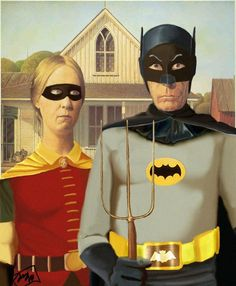
\includegraphics[width=0.5\textwidth,height=0.8\textheight]{img-batman.jpg}

\end{frame}

\begin{frame}\frametitle{Sensor Layout}
\begin{figure}
\centering
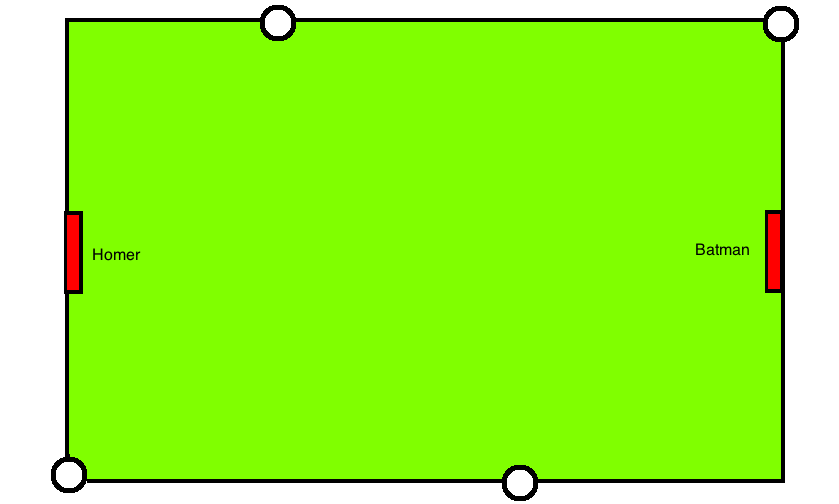
\includegraphics[scale=0.3]{layoutPic}
\caption{Width: 50cm, Length: 100cm}
\end{figure}
\end{frame}

\begin{frame}\frametitle{App Layout}
\begin{figure}
\centering
\frame{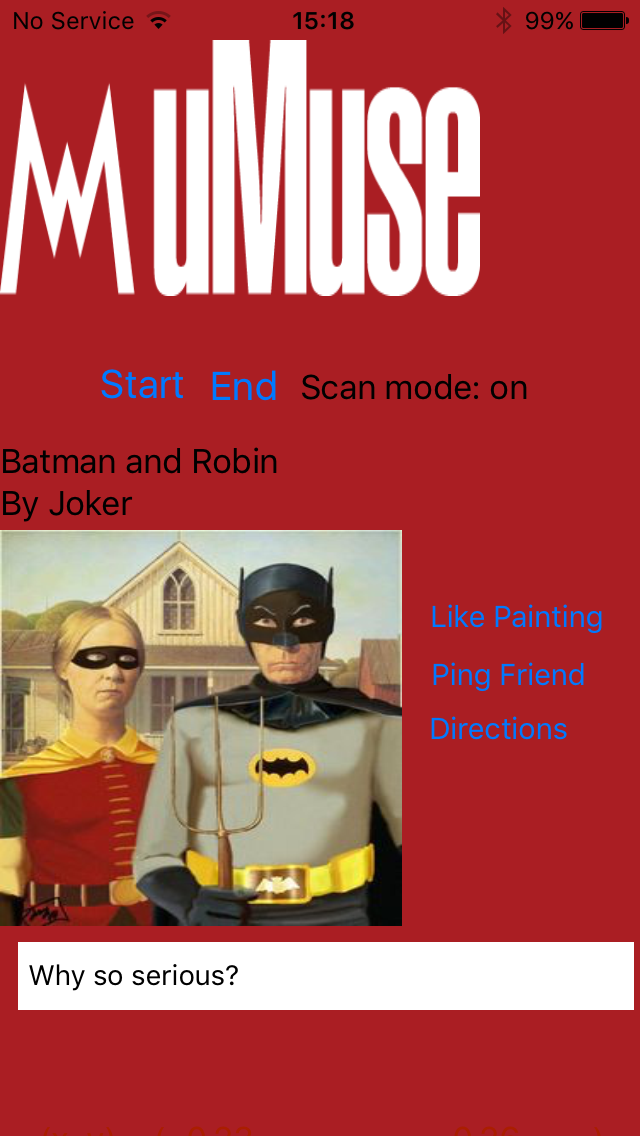
\includegraphics[scale=0.2]{appLayout}}
\end{figure}
\end{frame}

\begin{frame}[fragile]\frametitle{Main Program}
\begin{verbatim}
1  -(void) main:(NSObject *) RSSI {
2      NSObject RSSI_use = 
         [self discardMostDistantSensor(RSSI)];
3      double position = 
         [self getPosition: RSSI_use]; // x, y values
4      double dist2painting1 = 
         [self computeDistance: position: painting1];
5      double dist2painting2 = 
         [self computeDistance: position: painting2];
6      [self reportPosition2server: position];
7      int nearestPainting = 1;
8      if (dist2painting1 > dist2painting2) {
9          nearestPainting = 2;
10     }
11     [self updateImageViewer: nearestPainting];
12 }
\end{verbatim}
\end{frame}


\begin{frame}\frametitle{Integrating Machine Learning}
\begin{itemize}
\item Learn the most liked painting (not really ML)
\item Learn the most walked path.
\item Attempt to use walked paths to identify groups/couples.
\item Given a new painting with new path, use as indicator of paintings monetary value (new idea).
\end{itemize}
\end{frame}

\begin{frame}\frametitle{Kuo chat about:}
\begin{itemize}
\item stuff that Chris doesn't understand..
\item (Chris sets up and performs demo after Kuo finished)
\end{itemize}
\end{frame}

\begin{frame}\frametitle{Quick Demo}
\begin{figure}
\centering

\includegraphics[scale=2]{homer-crosses-fingers.jpg}
\end{figure}
\end{frame}


%%% Frame 2: NAG
%\begin{frame}\frametitle{NAG}
%	\center{\includegraphics[scale=0.5]{nag-logo}}
%\end{frame}
%%% -----------------
%
%
%%% Frame 3: Correlation Matrix
%\begin{frame}\frametitle{Correlation Matrix}
%	A \textit{Correlation Matrix} $A = [a_{ij}]\in\mathbb{R}^{n\times n}$ has the following properties
%	\begin{enumerate}
%		\item Symmetric, $A = A^T$
%		\item Non-negative eigenvalues, $\lambda_i(A) \geq 0$ $\forall$ $i = 1:n$
%		\item Unit-diagonal, $a_{ii} = 1$, $\forall$ $i = 1:n$
%	\end{enumerate}\pause
%	Note, a property of positive semi-definite matrices, 
%	\[
%		|a_{ij}|\leq\sqrt{a_{ii}a_{jj}}
%	\]
%	For a correlation matrix $a_{ii} = a_{jj} = 1$, therefore
%	\[
%		|a_{ij}|\leq 1 \Leftrightarrow a_{ij}\in[-1,1]
%	\]
%\end{frame}
%
%%% -----------------
%
%
%%%% Frame 4: Intuition of Correlation Matrix by Example 1
%%\begin{frame}\frametitle{Intuition of Correlation Matrices by Example}\framesubtitle{House Prices}
%%	\begin{columns}[T]
%%		\begin{column}{.5\textwidth}
%%			\begin{block}{}
%%				\includegraphics[scale=0.25]{house-price}
%%			\end{block}
%%		\end{column}\pause
%%		\begin{column}{.5\textwidth}
%%			Correlation Matrix for data
%%			\[
%%				A = \begin{pmatrix}1.0 & 0.958\\0.958 & 1.0\end{pmatrix}
%%			\]\pause
%%			$\lambda(A) = \{0.043, 1.958 \}$
%%		\end{column}
%%	\end{columns}	
%%\end{frame}
%%% -----------------
%
%
%%% Frame 5': Intuition of Correlation by Example 2
%\begin{frame}\frametitle{Intuition of Correlation Matrices by Example}\framesubtitle{Stock Market}
%	\begin{table}
%		\begin{tabular}{c | c | c | c | c}
%			Time & McDonalds & CocaCola & Apple & Nike \\
%			\hline \hline
% 			0    & 19        & 15       & 12    & 8    \\
% 			1    & 16        & 14       & 18    & 4    \\
%		    2    & 15        & 11       & 14    & 9    \\
%			3    & 11        & 14       & 4     & 10   \\
%			4    & 9         & 14       & 8     & 3    \\
%			5    & 17        & 14       & 10    & 12   \\
%      		6    & 19        & 13        & 20    & 5    \\
%			7    & 14        & 20       & 4     & 8    \\
%			8    & 20        & 14        & 18    & 12   \\
%			9    & 20        & 11        & 13    & 6
%		\end{tabular}
%	\end{table}
%\end{frame}
%
%%% Frame 5'': Intuition of Correlation by Example 2
%\begin{frame}\frametitle{Intuition of Correlation Matrices by Example}\framesubtitle{Stock Market}
%	\includegraphics[scale=0.5]{stock}
%\end{frame}
%
%%% Frame 5''': Intuition of Correlation by Example 2
%\begin{frame}\frametitle{Intuition by Example}\framesubtitle{Stock Market}
%	Correlation Matrix for the data
%	\[
%			A = \begin{blockarray}{ccccc}
%				       &  MD     & CC      & A       & N       \\
%			    \begin{block}{c(cccc)}
%			    	MD &  1.0    &  0.7139 &  0.4129 &  0.3496 \\
%  					CC &  0.7139 &  1.0    & -0.5795 & -0.1956 \\
%  					A  &  0.4129 & -0.5795 &  1.0    & -0.1717 \\
% 					N  &  0.3496 & -0.1956 & -0.1717 &  1.0    \\
%				\end{block}
%				\end{blockarray}
%	    \]
%	$\lambda(A) = \{1.9230, 0.2438, 0.6406, 1.1927\}$
%\end{frame}
%
%%% Frame 5"": Intuition of Correlation by Example 2
%\begin{frame}\frametitle{Intuition by Example}\framesubtitle{Stock Market}
%	\begin{table}
%		\begin{tabular}{c | c | c | c | c}
%			Time & McDonalds & CocaCola & Apple & Nike \\
%			\hline \hline
% 			0    & 19        &          & 12    & 8  \\
% 			1    & 16        & 14       &       & 4  \\
%		    2    & 15        &          & 14    & 9  \\
%			3    & 11        & 14       & 4     & 10 \\
%			4    &           & 14       & 8     & 3  \\
%			5    & 17        & 14       &       & 12 \\
%      		6    & 19        & 13       & 20    & 5  \\
%			7    & 14        & 20       & 4     &    \\
%			8    & 20        & 14       & 18    & 12 \\
%			9    & 20        &          & 13    & 6
%		\end{tabular}
%	\end{table}
%\end{frame}
%
%%% Frame 5""': Intuition of Correlation by Example 2
%\begin{frame}\frametitle{Intuition by Example}\framesubtitle{Stock Market}
%	Correlation Matrix for the data
%		\[
%			\hat{A} = \begin{blockarray}{ccccc}
%				      			 				   & MD     & CC               & A                & N      \\
%							\begin{block}{c(cccc)}
%  						 						MD &  1.0   & -0.851           & 0.752            &  0.308 \\
%  						 						CC & -0.851 &  1.0             & \textbf{-1.346} & -0.512 \\
%  						 						A  &  0.752 & \textbf{-1.346} & 1.0              &  0.051 \\
% 						 						N  &  0.308 & -0.512           & 0.051            &  1.0   \\
%							\end{block}
%					  \end{blockarray}
%	    \]
%
%	$\lambda(\hat{A}) = \{3.1122, 0.3467, \textbf{-0.4248}, 0.9659\}$
%\end{frame}
%%% -----------------
%
%
%%% Frame 6: Restoring Definiteness, NCM
%\begin{frame}\frametitle{Restoring Definiteness}\framesubtitle{Nearest Correlation Matrix}	
%		Given an indefinte estimate and symmetric $A$, compute
%		\[
%			\min_{X} ||A - X||_F
%		\]
%		such that $X$ is a correlation matrix.\pause\\
%		\vspace{0.5cm}
%	Current software
%	\begin{itemize}
%		\item \textbf{Alternating Projections} [\textit{Higham}, 2002] MATLAB Code: \href{http://nickhigham.wordpress.com/2013/02/ 13/the-nearest-correlation-matrix/}{http://nickhigham.wordpress.com/2013/02/ 13/the-nearest-correlation-matrix/}
%		\item \textbf{Newton Method} [\textit{Qi} and \textit{Sun}, 2006] NAG Library: \texttt{G02AA}, \texttt{G02AB}, \texttt{G02AE}, \texttt{G02AJ}.
%	\end{itemize}
%\end{frame}
%%% -----------------
%
%
%%% Frame 7: Restoring Definiteness, Shrinking
%\begin{frame}\frametitle{Restoring Definiteness}\framesubtitle{Shrinking [\textit{Higham}, \textit{Strabi\'{c}}, \textit{\u{S}ego}]}
%	\[
%		S(\alpha) = \alpha T + (1 - \alpha) A
%	\]
%	\begin{itemize}
%		\item Target matrix $T\in\mathbb{R}^{n\times n}$ (\textbf{chosen by user}).
%		\item Shrinking parameter $0\leq\alpha\leq 1$
%	\end{itemize}
%\end{frame}
%
%%% Frame 7': Restoring Definiteness, Shrinking
%\begin{frame}\frametitle{Restoring Definiteness}\framesubtitle{Shrinking [\textit{Higham}, \textit{Strabi\'{c}}, \textit{\u{S}ego}]}
%	Find the $\alpha^*$ that zero's the objective function $f: [0,1] \rightarrow \mathbb{R}$,
%	\[
%		f(\alpha) = \lambda_{min}(S(\alpha))
%	\]
%	$S(\alpha^*)$ is a correlation matrix.\pause
%	\begin{figure}
%		\includegraphics[scale=0.3]{min_eig_plot}\caption{Typical plot for $f(\alpha)$}
%	\end{figure}
%\end{frame}
%
%%% Frame 7'': Restoring Definiteness, Shrinking
%\begin{frame}\frametitle{Restoring Definiteness}\framesubtitle{Shrinking [\textit{Higham}, \textit{Strabi\'{c}}, \textit{\u{S}ego}]}
%	\textbf{Algorithm:} Compute optimal $\alpha^*$ with convergence tolerance $tol$
%	
%	\begin{algorithm}[H]
% $left = 0$; $right = 1$\;
% \While{$right - left > tol$}{
%  $mid = (left + right)/2$\;
%  \eIf{Cholesky factorisation of S(mid) fails}{
%   $left = mid$\;
%   }{
%   $right = mid$\;
%  }
% }
% $\alpha^* = right$\;
%\end{algorithm}
%
%Bisection converges in $N = \lceil\log_2(\sfrac{1}{tol})\rceil$ iterations.
%
%\end{frame}
%
%%% -----------------
%
%
%%% Frame 8: Shrinking
%\begin{frame}\frametitle{Shrinking}\framesubtitle{\texttt{G02AN}}
%	\[
%		T = \begin{pmatrix}
%				A_k & 0       \\
%				0   & I_{n-k}
%			\end{pmatrix},\text{ }
%		A = \begin{pmatrix}
%		    	A_k & Y       \\
%				Y^T & B
%		    \end{pmatrix}
%	\]
%	$A_k\in\mathbb{R}^{k\times k}$, $1 \leq k < n$ is \textbf{positive definite} and $B\in\mathbb{R}^{(n-k)\times (n-k)}$\pause
%	\begin{align*}
%		S(\alpha) & = \alpha\begin{pmatrix}A_k&0\\0&I_{n-k}\end{pmatrix}
%					   +(1-\alpha)\begin{pmatrix}A_k&Y\\Y^T&B\end{pmatrix}\\\\\pause
%				  & = \begin{pmatrix}
%				  	  	A_k 		  & (1-\alpha)Y\\
%				  	  	(1-\alpha)Y^T & \alpha I_{n-k} + (1-\alpha)B
%				      \end{pmatrix}	
%	\end{align*}
%\end{frame}
%
%%% Frame 8': Shrinking
%\begin{frame}\frametitle{Shrinking}\framesubtitle{\texttt{G02AN}}
%	Assume $\alpha > \alpha^*$ $\Rightarrow 0 < S(\alpha) = R^TR$, where $R = \begin{pmatrix}R_{11}&R_{12}\\0&R_{22}\end{pmatrix}$\pause , so
%	\begin{align*}
%		S(\alpha) & = \begin{pmatrix}
%				  	  	A_k 		  & (1-\alpha)Y\\
%				  	  	(1-\alpha)Y^T & \alpha I_{n-k} + (1-\alpha)B
%				      \end{pmatrix}\\ & = R^TR = \begin{pmatrix}R_{11}^T&0\\R_{12}^T&R_{22}^T\end{pmatrix}\begin{pmatrix}R_{11}&R_{12}\\0&R_{22}\end{pmatrix}\\
%		& = \begin{pmatrix}
%			R_{11}^TR_{11}&R_{11}^TR_{12}\\R_{12}^TR_{11}&R_{12}^TR_{12} + R_{22}^TR_{22}		    
%		    \end{pmatrix}				
%	\end{align*}\pause
%	\begin{align*}
%		& \Rightarrow R_{11}^TR_{11} = A_k\text{, $R_{11}$ is the Cholesky factor of $A_k$}\\
%		& \Rightarrow R_{11}^TR_{12} = (1-\alpha)Y \Leftrightarrow R_{12} = (1-\alpha)(R_{11}^T)^{-1}Y\\
%		& \Rightarrow R_{12}^TR_{12} + R_{22}^TR_{22} = \alpha I_{n-k} + (1-\alpha)B \\
%		& \hspace{0.5cm} \Leftrightarrow R_{22}^TR_{22} = \alpha I_{n-k} + (1-\alpha)B - R_{12}^TR_{12}\hspace{1.5cm}(*)
%	\end{align*}
%\end{frame}
%
%\begin{frame}\frametitle{Shrinking}\framesubtitle{\texttt{G02AN}}
%Define $P(\alpha)\in\mathbb{R}^{(n-k)\times (n-k)}$,
%	\[
%		P(\alpha) = \alpha I_{n-k} + (1-\alpha)B - (1-\alpha)^2Z
%	\]
%	where $Z = Y^T((R_{11}^T)^{-1})^T(R_{11}^T)^{-1}Y$
%\end{frame}
%
%
%%% Frame 8'': Shrinking
%\begin{frame}\frametitle{Shrinking}\framesubtitle{\texttt{G02AN}}\pause
%	\textbf{Algorithm:} \texttt{G02AN}
%	\begin{algorithm}[H]
% $left = 0$; $right = 1$\;
% $R_{11} = \texttt{chol}(A_k)$; $G = R_{11}^T \backslash Y$; $Z = G^TG$\;
% \While{$right - left > tol$}{
%  $mid = (left + right)/2$\;
%  \eIf{Cholesky factorisation of $P(mid)$ fails}{
%   $left = mid$\;
%   }{
%   $right = mid$\;
%  }
% }
% $\alpha^* = right$\;
%\end{algorithm}
%\end{frame}
%
%%% Frame 9: Numerical Experiments
%\begin{frame}\frametitle{Numerical Experiments}\framesubtitle{NCM vs. Shrink vs. Shrink\_FB}
%	\vspace{-0.6cm}	
%	\begin{figure}
%		\includegraphics[scale=0.5]{Compare_graph1}\caption{Tests performed on Windows running MATLAB R2014a with Intel Core 2 Quad CPU 2.83GHz and 4.00GB RAM}
%	\end{figure}
%	Tolerance set at $10^{-6}$ and note NCM uses \texttt{G02AA}.
%\end{frame}
%
%%% Frame 9': Numerical Experiments
%\begin{frame}\frametitle{Numerical Experiments}\framesubtitle{Shrink vs. Shrink\_FB}
%	\begin{figure}
%		\includegraphics[scale=0.5]{Compare_graph2}\caption{Tests performed on Windows running MATLAB R2014a with Intel Core 2 Quad CPU 2.83GHz and 4.00GB RAM}
%	\end{figure}
%\end{frame}
%
%%% Frame 9'': Numerical Experiments
%\begin{frame}\frametitle{Numerical Experiments}\framesubtitle{Relative difference in time: NCM vs. Shrink}
%	\begin{figure}
%		\includegraphics[scale=0.5]{rel_dif_graph}
%	\end{figure}
%	\[
%		rel\_diff_i = 100\times\frac{NCM_i - Shrink_i}{NCM_i}
%	\]
%\end{frame}
%
%%% Frame 10: Furture work
%\begin{frame}\frametitle{Future Work}
%\begin{itemize}
%	\item Analysis of the effects of different target matrices, 
%	\item Study matrices with computable NCM and Shrinking distances (e.g. Tridiagonal Toeplitz Matrix), 
%	\item Fortran implementations of the alternating projections algorithm and shrinking with weighting for potential new NAG routines,
%	\item Generalise the theory to Covariance matrices,
%	\item Compare new methods with current NAG code. 
%\end{itemize}
%\end{frame}

\begin{frame}
	Thank you for listening!\\Any Questions?
\end{frame}


\end{document}
